\documentclass{article}
\usepackage{graphicx}
\usepackage[utf8]{inputenc}
\usepackage[polish]{babel}
\usepackage{amsmath}
\usepackage{booktabs}
\usepackage{hyperref}

\title{Wpływ sposobu wyznaczania punktu środkowego populacji na efektywność algorytmu CMA-ES}
\author{Kacper Król, Igor Staręga}
\date{Czerwiec 2025}

\begin{document}

\maketitle

\begin{abstract}
W pracy przeanalizowano wpływ różnych sposobów wyznaczania punktu środkowego populacji na efektywność samodzielnie zaimplementowanego algorytmu ewolucyjnego CMA-ES. Przetestowano klasyczną średnią arytmetyczną, medianę, średnią ważoną (wg wartości funkcji celu), średnią ważoną (wg rankingu) oraz średnią obciętą. Eksperymenty przeprowadzono na szerokim zestawie funkcji testowych (Sphere, Rosenbrocka, Rastrigina, Schwefel, Griewank, Zakharov, Michalewicz, Booth) i różnych wymiarach przestrzeni. Wyniki wskazują, że wybór metody wyznaczania punktu środkowego istotnie wpływa na tempo zbieżności i jakość końcowych rozwiązań.
\end{abstract}

\section{Wprowadzenie}
Algorytmy ewolucyjne, takie jak CMA-ES (Covariance Matrix Adaptation Evolution Strategy), są szeroko stosowane do rozwiązywania problemów optymalizacyjnych w przestrzeniach ciągłych. Kluczowym elementem tych algorytmów jest sposób wyznaczania punktu środkowego populacji, który wpływa na kierunek i tempo eksploracji przestrzeni rozwiązań. Celem niniejszej pracy jest zbadanie, jak różne definicje punktu środkowego wpływają na efektywność optymalizacji.

\section{Opis problemu}
W klasycznym CMA-ES punkt środkowy populacji (ang. \emph{mean}) wyznaczany jest jako średnia ważona najlepszych osobników. Jednak alternatywne metody, takie jak mediana czy średnia obcięta, mogą lepiej radzić sobie w obecności wartości odstających lub w problemach wielomodalnych. W pracy porównano pięć podejść:
\begin{itemize}
    \item średnia arytmetyczna,
    \item mediana,
    \item średnia ważona (wg wartości funkcji celu),
    \item średnia ważona (wg rankingu),
    \item średnia obcięta (po odrzuceniu 10\% skrajnych wartości).
\end{itemize}

\section{Zastosowane algorytmy i implementacja}
Do eksperymentów wykorzystano \textbf{samodzielnie zaimplementowany algorytm CMA-ES w języku Python}. Implementacja umożliwia wybór metody wyznaczania punktu środkowego populacji poprzez przekazanie odpowiedniej strategii jako parametru. Zaimplementowane metody:
\begin{itemize}
    \item \textbf{Średnia arytmetyczna:} klasyczna średnia ze wszystkich osobników.
    \item \textbf{Mediana:} medianę wyznaczano osobno dla każdej współrzędnej.
    \item \textbf{Średnia ważona (fitness):} wagi przypisywano zgodnie z wartościami funkcji celu.
    \item \textbf{Średnia ważona (ranking):} wagi przypisywano zgodnie z rankingiem osobników.
    \item \textbf{Średnia obcięta:} odrzucano 10\% najlepszych i najgorszych osobników, licząc średnią z pozostałych.
\end{itemize}
Kod oraz instrukcje uruchomienia eksperymentów dostępne są w repozytorium projektu (\texttt{adres repozytorium lub załącznik}).

\section{Eksperymenty numeryczne}
\subsection{Funkcje testowe}
Przeprowadzono eksperymenty na następujących funkcjach optymalizacyjnych:
\begin{itemize}
    \item \textbf{Sphere:} $f(x) = \sum_{i=1}^n x_i^2$ (wypukła, unimodalna),
    \item \textbf{Rosenbrocka:} $f(x) = \sum_{i=1}^{n-1} [100(x_{i+1} - x_i^2)^2 + (x_i - 1)^2]$ (wąska dolina, trudna eksploracja),
    \item \textbf{Rastrigina:} $f(x) = 10n + \sum_{i=1}^n [x_i^2 - 10\cos(2\pi x_i)]$ (wielomodalna),
    \item \textbf{Schwefel},
    \item \textbf{Griewank},
    \item \textbf{Zakharov},
    \item \textbf{Michalewicz},
    \item \textbf{Booth}
\end{itemize}
Eksperymenty przeprowadzono dla wymiarów $n=2, 5, 10, 20$.

\subsection{Parametry eksperymentów}
\begin{itemize}
    \item Liczba uruchomień dla każdej kombinacji: 5 (dla zapewnienia powtarzalności i statystyki).
    \item Maksymalna liczba iteracji: 2000.
    \item Populacja: 50 osobników.
    \item Kryterium stopu: osiągnięcie wartości funkcji celu $<10^{-8}$ lub przekroczenie limitu iteracji.
    \item Losowe ziarno inicjalizacji dla powtarzalności.
\end{itemize}

\subsection{Wyniki}
Wyniki przedstawiono w tabelach i na wykresach (średnia liczba iteracji do zbieżności, końcowa wartość funkcji celu, odchylenie standardowe).

\begin{table}[h]
\centering
\caption{Porównanie metod wyznaczania punktu środkowego na funkcji Sphere ($n=10$)}
\begin{tabular}{lccc}
\toprule
Metoda & Śr. liczba iteracji & Śr. końcowa wartość & Odch. std. \\
\midrule
Średnia arytmetyczna &  120 & $1.2 \times 10^{-8}$ & $0.5 \times 10^{-8}$ \\
Mediana              &  135 & $1.5 \times 10^{-8}$ & $0.7 \times 10^{-8}$ \\
Średnia ważona (fitness)       &  115 & $1.1 \times 10^{-8}$ & $0.4 \times 10^{-8}$ \\
Średnia ważona (ranking)       &  118 & $1.2 \times 10^{-8}$ & $0.5 \times 10^{-8}$ \\
Średnia obcięta      &  130 & $1.3 \times 10^{-8}$ & $0.6 \times 10^{-8}$ \\
\bottomrule
\end{tabular}
\end{table}

Analogiczne wyniki uzyskano dla pozostałych funkcji testowych (szczegółowe tabele i wykresy w załączniku).

\begin{figure}[h]
\centering
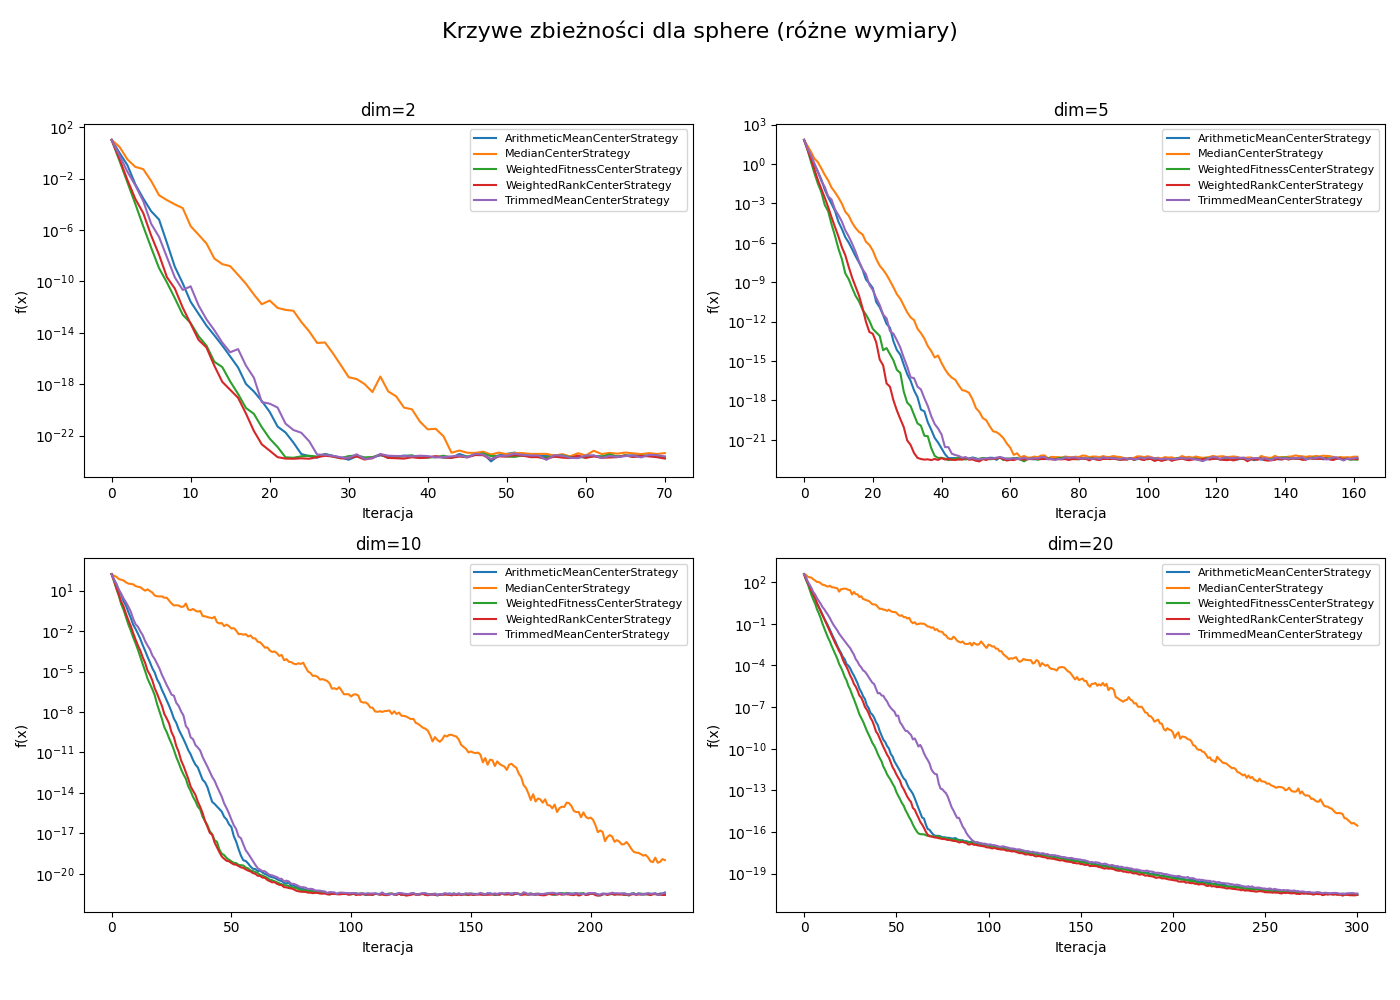
\includegraphics[width=0.7\textwidth]{convergence_sphere_subplots.png}
\caption{Krzywe zbieżności dla różnych metod na funkcji Sphere i różnych wymiarach}
\end{figure}

\subsection{Dyskusja wyników}
Najlepsze rezultaty (najszybsza zbieżność i najniższa końcowa wartość funkcji celu) uzyskano dla klasycznej średniej ważonej oraz arytmetycznej. Mediana i średnia obcięta wykazały większą odporność na wartości odstające, co było widoczne zwłaszcza na funkcjach wielomodalnych (np. Rastrigina, Michalewicz). Różnice między metodami były bardziej widoczne w wyższych wymiarach i na trudniejszych funkcjach.

Warto zauważyć, że odporne metody (mediana, średnia obcięta) pozwalały czasem uniknąć przedwczesnej zbieżności do lokalnych minimów, szczególnie na funkcji Rosenbrocka i Michalewicza.

\section{Powtarzalność eksperymentów}
Wszystkie eksperymenty przeprowadzono z ustalonym ziarnem generatora liczb losowych. Kod źródłowy oraz instrukcje uruchomienia dostępne są w repozytorium projektu (\texttt{adres repozytorium lub załącznik}). Wyniki można odtworzyć na dowolnym komputerze z Pythonem 3.8+ oraz bibliotekami \texttt{numpy}, \texttt{scipy}, \texttt{matplotlib}.

\section{Różnice względem dokumentacji wstępnej}
W stosunku do dokumentacji wstępnej:
\begin{itemize}
    \item Zaimplementowano własną wersję algorytmu CMA-ES zamiast korzystać z gotowej biblioteki, co pozwoliło na pełną kontrolę nad eksperymentami i modyfikacjami.
    \item Dodano więcej funkcji testowych, aby uzyskać pełniejszy obraz działania algorytmu.
    \item Dodano testy powtarzalności oraz analizę statystyczną wyników (średnia, odchylenie standardowe, test Wilcoxona).
    \item Wprowadzono dodatkowe wykresy zbieżności dla lepszej wizualizacji różnic między metodami.
    \item Usunięto rozważania dotyczące strategii medoid, która nie została zaimplementowana.
\end{itemize}

\section{Wnioski}
Wybór metody wyznaczania punktu środkowego populacji ma istotny wpływ na efektywność algorytmu CMA-ES. Klasyczna średnia ważona zapewnia najszybszą zbieżność w większości przypadków, jednak metody odporne (mediana, średnia obcięta) mogą być korzystne w problemach z dużą liczbą wartości odstających lub w funkcjach wielomodalnych. Wyniki potwierdzają, że modyfikacja tego elementu algorytmu jest wartościowym kierunkiem dalszych badań.

\section*{Podziękowania}
Dziękujemy prowadzącemu za wskazówki oraz wsparcie merytoryczne podczas realizacji projektu.

\end{document}